\documentclass{standalone}
\usepackage{tikz}
\usetikzlibrary{patterns, positioning}

\begin{document}
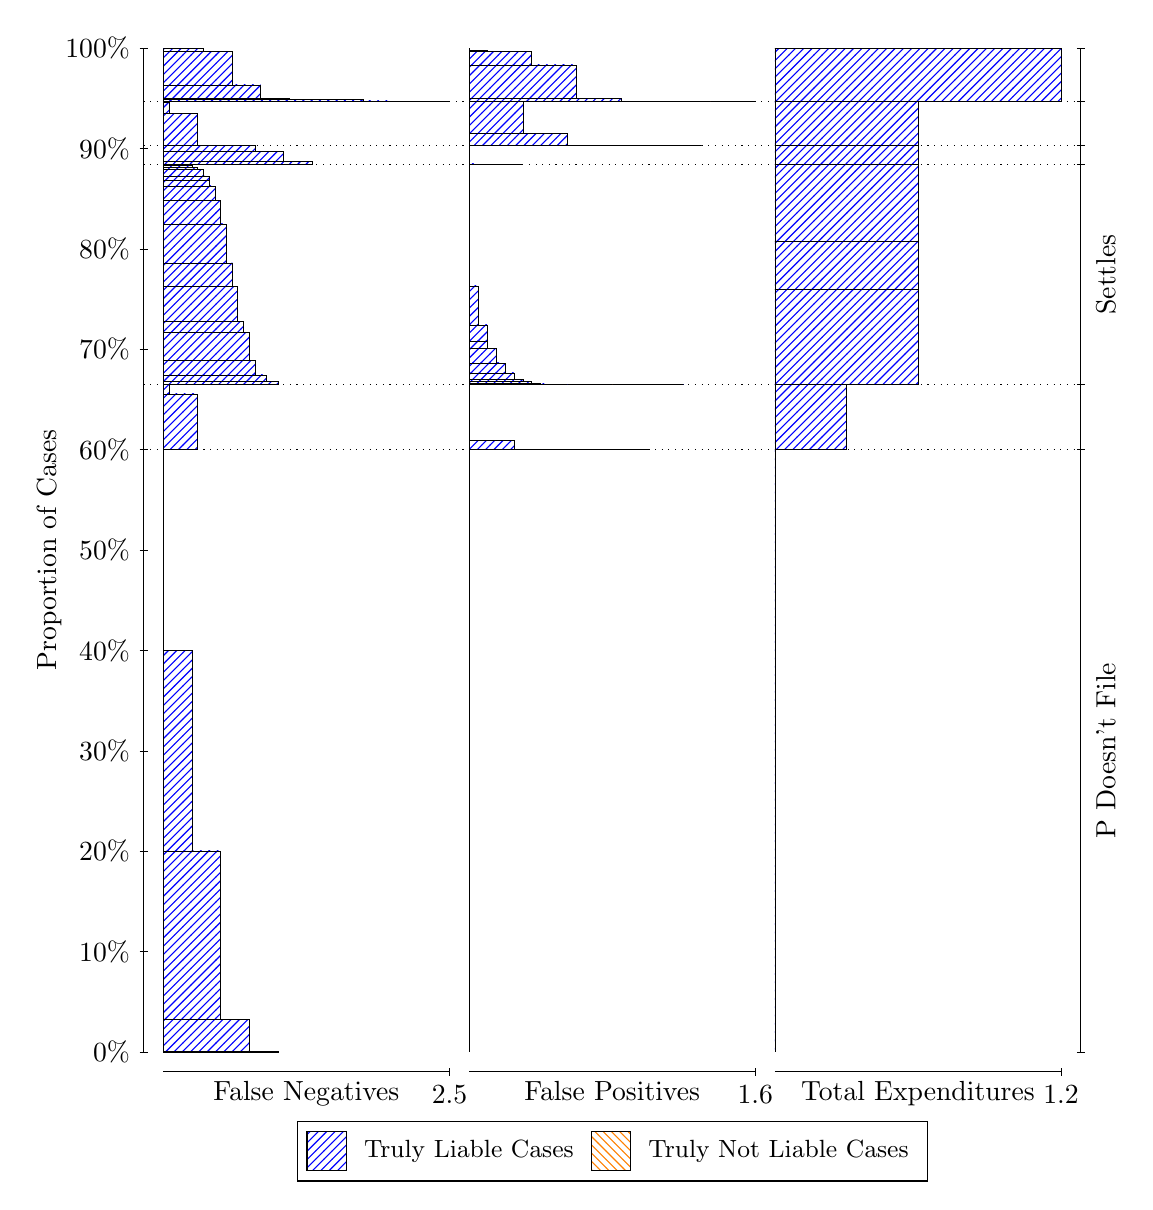
\begin{tikzpicture}
\draw[black, very thin] (1.5,1.75) -- (1.5,14.5);
\node[rotate=90, anchor=center] at (0.3, 8.125) {Proportion of Cases};
\draw[black, very thin] (1.45,1.75) -- (1.55,1.75);
\node[anchor=east] at (1.45, 1.75) {0\%};
\draw[black, very thin] (1.45,3.025) -- (1.55,3.025);
\node[anchor=east] at (1.45, 3.025) {10\%};
\draw[black, very thin] (1.45,4.3) -- (1.55,4.3);
\node[anchor=east] at (1.45, 4.3) {20\%};
\draw[black, very thin] (1.45,5.575) -- (1.55,5.575);
\node[anchor=east] at (1.45, 5.575) {30\%};
\draw[black, very thin] (1.45,6.85) -- (1.55,6.85);
\node[anchor=east] at (1.45, 6.85) {40\%};
\draw[black, very thin] (1.45,8.125) -- (1.55,8.125);
\node[anchor=east] at (1.45, 8.125) {50\%};
\draw[black, very thin] (1.45,9.4) -- (1.55,9.4);
\node[anchor=east] at (1.45, 9.4) {60\%};
\draw[black, very thin] (1.45,10.675) -- (1.55,10.675);
\node[anchor=east] at (1.45, 10.675) {70\%};
\draw[black, very thin] (1.45,11.95) -- (1.55,11.95);
\node[anchor=east] at (1.45, 11.95) {80\%};
\draw[black, very thin] (1.45,13.225) -- (1.55,13.225);
\node[anchor=east] at (1.45, 13.225) {90\%};
\draw[black, very thin] (1.45,14.5) -- (1.55,14.5);
\node[anchor=east] at (1.45, 14.5) {100\%};

\draw[black, very thin] (13.4,1.75) -- (13.4,14.5);
\draw[black, very thin] (13.35,1.75) -- (13.45,1.75);
\node[anchor=west] at (13.35, 1.75) {};
\draw[black, very thin] (13.35,9.4013) -- (13.45,9.4013);
\node[anchor=west] at (13.35, 9.4013) {};
\draw[black, very thin] (13.35,10.224) -- (13.45,10.224);
\node[anchor=west] at (13.35, 10.224) {};
\draw[black, very thin] (13.35,13.026) -- (13.45,13.026);
\node[anchor=west] at (13.35, 13.026) {};
\draw[black, very thin] (13.35,13.263) -- (13.45,13.263);
\node[anchor=west] at (13.35, 13.263) {};
\draw[black, very thin] (13.35,13.818) -- (13.45,13.818);
\node[anchor=west] at (13.35, 13.818) {};
\draw[black, very thin] (13.35,14.5) -- (13.45,14.5);
\node[anchor=west] at (13.35, 14.5) {};

\draw[black, very thin, pattern color=blue, pattern=north east lines] (1.75,1.75) rectangle (3.2033,1.7541);
\draw[black, very thin, pattern color=blue, pattern=north east lines] (1.75,1.7541) rectangle (2.84,2.1592);
\draw[black, very thin, pattern color=blue, pattern=north east lines] (1.75,2.1592) rectangle (2.4767,4.3047);
\draw[black, very thin, pattern color=blue, pattern=north east lines] (1.75,4.3047) rectangle (2.1133,6.8513);
\draw[black, very thin, pattern color=orange, pattern=north west lines] (1.75,6.8513) rectangle (1.75,6.8513);
\draw[black, very thin, pattern color=blue, pattern=north east lines] (1.75,6.8513) rectangle (1.75,9.4013);
\draw[black, very thin, pattern color=blue, pattern=north east lines] (1.75,9.4013) rectangle (2.186,10.109);
\draw[black, very thin, pattern color=blue, pattern=north east lines] (1.75,10.109) rectangle (1.8227,10.224);
\draw[black, very thin, pattern color=orange, pattern=north west lines] (1.75,10.224) rectangle (1.75,10.224);
\draw[black, very thin, pattern color=blue, pattern=north east lines] (1.75,10.224) rectangle (1.75,10.224);
\draw[black, very thin, pattern color=blue, pattern=north east lines] (1.75,10.224) rectangle (3.2033,10.268);
\draw[black, very thin, pattern color=blue, pattern=north east lines] (1.75,10.268) rectangle (3.058,10.348);
\draw[black, very thin, pattern color=blue, pattern=north east lines] (1.75,10.348) rectangle (2.9127,10.532);
\draw[black, very thin, pattern color=blue, pattern=north east lines] (1.75,10.532) rectangle (2.84,10.888);
\draw[black, very thin, pattern color=blue, pattern=north east lines] (1.75,10.888) rectangle (2.7673,11.03);
\draw[black, very thin, pattern color=blue, pattern=north east lines] (1.75,11.03) rectangle (2.6947,11.468);
\draw[black, very thin, pattern color=blue, pattern=north east lines] (1.75,11.468) rectangle (2.622,11.771);
\draw[black, very thin, pattern color=blue, pattern=north east lines] (1.75,11.771) rectangle (2.5493,12.267);
\draw[black, very thin, pattern color=blue, pattern=north east lines] (1.75,12.267) rectangle (2.4767,12.569);
\draw[black, very thin, pattern color=blue, pattern=north east lines] (1.75,12.569) rectangle (2.404,12.75);
\draw[black, very thin, pattern color=blue, pattern=north east lines] (1.75,12.75) rectangle (2.3313,12.817);
\draw[black, very thin, pattern color=blue, pattern=north east lines] (1.75,12.817) rectangle (2.3313,12.877);
\draw[black, very thin, pattern color=blue, pattern=north east lines] (1.75,12.877) rectangle (2.2587,12.96);
\draw[black, very thin, pattern color=blue, pattern=north east lines] (1.75,12.96) rectangle (2.186,12.987);
\draw[black, very thin, pattern color=blue, pattern=north east lines] (1.75,12.987) rectangle (2.1133,13.007);
\draw[black, very thin, pattern color=blue, pattern=north east lines] (1.75,13.007) rectangle (2.0407,13.015);
\draw[black, very thin, pattern color=blue, pattern=north east lines] (1.75,13.015) rectangle (1.968,13.015);
\draw[black, very thin, pattern color=blue, pattern=north east lines] (1.75,13.015) rectangle (1.968,13.025);
\draw[black, very thin, pattern color=blue, pattern=north east lines] (1.75,13.025) rectangle (1.8953,13.026);
\draw[black, very thin, pattern color=blue, pattern=north east lines] (1.75,13.026) rectangle (1.8227,13.026);
\draw[black, very thin, pattern color=orange, pattern=north west lines] (1.75,13.026) rectangle (1.75,13.026);
\draw[black, very thin, pattern color=blue, pattern=north east lines] (1.75,13.026) rectangle (1.75,13.026);
\draw[black, very thin, pattern color=blue, pattern=north east lines] (1.75,13.026) rectangle (3.6393,13.059);
\draw[black, very thin, pattern color=blue, pattern=north east lines] (1.75,13.059) rectangle (3.276,13.185);
\draw[black, very thin, pattern color=blue, pattern=north east lines] (1.75,13.185) rectangle (2.9127,13.261);
\draw[black, very thin, pattern color=blue, pattern=north east lines] (1.75,13.261) rectangle (2.5493,13.263);
\draw[black, very thin, pattern color=blue, pattern=north east lines] (1.75,13.263) rectangle (2.186,13.263);
\draw[black, very thin, pattern color=orange, pattern=north west lines] (1.75,13.263) rectangle (1.75,13.263);
\draw[black, very thin, pattern color=blue, pattern=north east lines] (1.75,13.263) rectangle (2.186,13.668);
\draw[black, very thin, pattern color=blue, pattern=north east lines] (1.75,13.668) rectangle (1.8227,13.814);
\draw[black, very thin, pattern color=orange, pattern=north west lines] (1.75,13.814) rectangle (1.75,13.814);
\draw[black, very thin, pattern color=blue, pattern=north east lines] (1.75,13.814) rectangle (1.75,13.818);
\draw[black, very thin, pattern color=blue, pattern=north east lines] (1.75,13.818) rectangle (5.3833,13.818);
\draw[black, very thin, pattern color=blue, pattern=north east lines] (1.75,13.818) rectangle (5.02,13.818);
\draw[black, very thin, pattern color=blue, pattern=north east lines] (1.75,13.818) rectangle (4.6567,13.83);
\draw[black, very thin, pattern color=blue, pattern=north east lines] (1.75,13.83) rectangle (4.2933,13.85);
\draw[black, very thin, pattern color=blue, pattern=north east lines] (1.75,13.85) rectangle (3.93,13.851);
\draw[black, very thin, pattern color=blue, pattern=north east lines] (1.75,13.851) rectangle (3.712,13.851);
\draw[black, very thin, pattern color=blue, pattern=north east lines] (1.75,13.851) rectangle (3.5667,13.851);
\draw[black, very thin, pattern color=blue, pattern=north east lines] (1.75,13.851) rectangle (3.3487,13.857);
\draw[black, very thin, pattern color=blue, pattern=north east lines] (1.75,13.857) rectangle (3.2033,13.857);
\draw[black, very thin, pattern color=blue, pattern=north east lines] (1.75,13.857) rectangle (2.9853,14.033);
\draw[black, very thin, pattern color=blue, pattern=north east lines] (1.75,14.033) rectangle (2.622,14.455);
\draw[black, very thin, pattern color=blue, pattern=north east lines] (1.75,14.455) rectangle (2.2587,14.5);
\draw[black, very thin, pattern color=blue, pattern=north east lines] (1.75,14.5) rectangle (1.8953,14.5);
\draw[black, very thin, pattern color=orange, pattern=north west lines] (1.75,14.5) rectangle (1.75,14.5);
\draw[black, very thin, pattern color=blue, pattern=north east lines] (1.75,14.5) rectangle (1.75,14.5);
\draw[black, very thin, pattern color=orange, pattern=north west lines] (5.6333,1.75) rectangle (5.6333,1.75);
\draw[black, very thin, pattern color=blue, pattern=north east lines] (5.6333,1.75) rectangle (5.6333,9.4013);
\draw[black, very thin, pattern color=orange, pattern=north west lines] (5.6333,9.4013) rectangle (7.9042,9.4013);
\draw[black, very thin, pattern color=blue, pattern=north east lines] (5.6333,9.4013) rectangle (7.9042,9.4013);
\draw[black, very thin, pattern color=blue, pattern=north east lines] (5.6333,9.4013) rectangle (7.3365,9.4013);
\draw[black, very thin, pattern color=blue, pattern=north east lines] (5.6333,9.4013) rectangle (6.7687,9.4015);
\draw[black, very thin, pattern color=blue, pattern=north east lines] (5.6333,9.4015) rectangle (6.201,9.5171);
\draw[black, very thin, pattern color=blue, pattern=north east lines] (5.6333,9.5171) rectangle (5.6333,10.224);
\draw[black, very thin, pattern color=orange, pattern=north west lines] (5.6333,10.224) rectangle (8.3583,10.224);
\draw[black, very thin, pattern color=blue, pattern=north east lines] (5.6333,10.224) rectangle (8.3583,10.224);
\draw[black, very thin, pattern color=orange, pattern=north west lines] (5.6333,10.224) rectangle (8.1313,10.224);
\draw[black, very thin, pattern color=blue, pattern=north east lines] (5.6333,10.224) rectangle (8.1313,10.224);
\draw[black, very thin, pattern color=orange, pattern=north west lines] (5.6333,10.224) rectangle (7.9042,10.224);
\draw[black, very thin, pattern color=blue, pattern=north east lines] (5.6333,10.224) rectangle (7.9042,10.224);
\draw[black, very thin, pattern color=blue, pattern=north east lines] (5.6333,10.224) rectangle (7.7906,10.224);
\draw[black, very thin, pattern color=orange, pattern=north west lines] (5.6333,10.224) rectangle (7.6771,10.224);
\draw[black, very thin, pattern color=blue, pattern=north east lines] (5.6333,10.224) rectangle (7.6771,10.224);
\draw[black, very thin, pattern color=blue, pattern=north east lines] (5.6333,10.224) rectangle (7.5635,10.224);
\draw[black, very thin, pattern color=orange, pattern=north west lines] (5.6333,10.224) rectangle (7.45,10.224);
\draw[black, very thin, pattern color=blue, pattern=north east lines] (5.6333,10.224) rectangle (7.45,10.224);
\draw[black, very thin, pattern color=blue, pattern=north east lines] (5.6333,10.224) rectangle (7.3365,10.224);
\draw[black, very thin, pattern color=orange, pattern=north west lines] (5.6333,10.224) rectangle (7.2229,10.224);
\draw[black, very thin, pattern color=blue, pattern=north east lines] (5.6333,10.224) rectangle (7.2229,10.225);
\draw[black, very thin, pattern color=blue, pattern=north east lines] (5.6333,10.225) rectangle (7.1094,10.225);
\draw[black, very thin, pattern color=blue, pattern=north east lines] (5.6333,10.225) rectangle (6.9958,10.225);
\draw[black, very thin, pattern color=orange, pattern=north west lines] (5.6333,10.225) rectangle (6.9958,10.225);
\draw[black, very thin, pattern color=blue, pattern=north east lines] (5.6333,10.225) rectangle (6.9958,10.225);
\draw[black, very thin, pattern color=blue, pattern=north east lines] (5.6333,10.225) rectangle (6.8823,10.225);
\draw[black, very thin, pattern color=blue, pattern=north east lines] (5.6333,10.225) rectangle (6.7687,10.226);
\draw[black, very thin, pattern color=blue, pattern=north east lines] (5.6333,10.226) rectangle (6.6552,10.236);
\draw[black, very thin, pattern color=blue, pattern=north east lines] (5.6333,10.236) rectangle (6.5417,10.244);
\draw[black, very thin, pattern color=blue, pattern=north east lines] (5.6333,10.244) rectangle (6.4281,10.264);
\draw[black, very thin, pattern color=blue, pattern=north east lines] (5.6333,10.264) rectangle (6.4281,10.264);
\draw[black, very thin, pattern color=blue, pattern=north east lines] (5.6333,10.264) rectangle (6.3146,10.291);
\draw[black, very thin, pattern color=blue, pattern=north east lines] (5.6333,10.291) rectangle (6.201,10.374);
\draw[black, very thin, pattern color=blue, pattern=north east lines] (5.6333,10.374) rectangle (6.0875,10.501);
\draw[black, very thin, pattern color=blue, pattern=north east lines] (5.6333,10.501) rectangle (5.974,10.681);
\draw[black, very thin, pattern color=blue, pattern=north east lines] (5.6333,10.681) rectangle (5.8604,10.78);
\draw[black, very thin, pattern color=blue, pattern=north east lines] (5.6333,10.78) rectangle (5.8604,10.984);
\draw[black, very thin, pattern color=blue, pattern=north east lines] (5.6333,10.984) rectangle (5.7469,11.48);
\draw[black, very thin, pattern color=blue, pattern=north east lines] (5.6333,11.48) rectangle (5.6333,13.026);
\draw[black, very thin, pattern color=orange, pattern=north west lines] (5.6333,13.026) rectangle (6.3146,13.026);
\draw[black, very thin, pattern color=blue, pattern=north east lines] (5.6333,13.026) rectangle (6.3146,13.026);
\draw[black, very thin, pattern color=blue, pattern=north east lines] (5.6333,13.026) rectangle (5.7469,13.029);
\draw[black, very thin, pattern color=blue, pattern=north east lines] (5.6333,13.029) rectangle (5.6333,13.263);
\draw[black, very thin, pattern color=orange, pattern=north west lines] (5.6333,13.263) rectangle (8.5854,13.263);
\draw[black, very thin, pattern color=blue, pattern=north east lines] (5.6333,13.263) rectangle (8.5854,13.263);
\draw[black, very thin, pattern color=blue, pattern=north east lines] (5.6333,13.263) rectangle (8.0177,13.263);
\draw[black, very thin, pattern color=blue, pattern=north east lines] (5.6333,13.263) rectangle (7.45,13.267);
\draw[black, very thin, pattern color=blue, pattern=north east lines] (5.6333,13.267) rectangle (6.8823,13.413);
\draw[black, very thin, pattern color=blue, pattern=north east lines] (5.6333,13.413) rectangle (6.3146,13.818);
\draw[black, very thin, pattern color=orange, pattern=north west lines] (5.6333,13.818) rectangle (9.2667,13.818);
\draw[black, very thin, pattern color=blue, pattern=north east lines] (5.6333,13.818) rectangle (9.2667,13.818);
\draw[black, very thin, pattern color=orange, pattern=north west lines] (5.6333,13.818) rectangle (8.699,13.818);
\draw[black, very thin, pattern color=blue, pattern=north east lines] (5.6333,13.818) rectangle (8.699,13.818);
\draw[black, very thin, pattern color=orange, pattern=north west lines] (5.6333,13.818) rectangle (8.1313,13.818);
\draw[black, very thin, pattern color=blue, pattern=north east lines] (5.6333,13.818) rectangle (8.1313,13.818);
\draw[black, very thin, pattern color=blue, pattern=north east lines] (5.6333,13.818) rectangle (7.5635,13.863);
\draw[black, very thin, pattern color=orange, pattern=north west lines] (5.6333,13.863) rectangle (7.5635,13.863);
\draw[black, very thin, pattern color=blue, pattern=north east lines] (5.6333,13.863) rectangle (7.5635,13.863);
\draw[black, very thin, pattern color=blue, pattern=north east lines] (5.6333,13.863) rectangle (6.9958,14.284);
\draw[black, very thin, pattern color=blue, pattern=north east lines] (5.6333,14.284) rectangle (6.9958,14.285);
\draw[black, very thin, pattern color=blue, pattern=north east lines] (5.6333,14.285) rectangle (6.4281,14.458);
\draw[black, very thin, pattern color=blue, pattern=north east lines] (5.6333,14.458) rectangle (6.4281,14.46);
\draw[black, very thin, pattern color=orange, pattern=north west lines] (5.6333,14.46) rectangle (6.0875,14.46);
\draw[black, very thin, pattern color=blue, pattern=north east lines] (5.6333,14.46) rectangle (6.0875,14.46);
\draw[black, very thin, pattern color=blue, pattern=north east lines] (5.6333,14.46) rectangle (5.8604,14.467);
\draw[black, very thin, pattern color=blue, pattern=north east lines] (5.6333,14.467) rectangle (5.8604,14.467);
\draw[black, very thin, pattern color=orange, pattern=north west lines] (5.6333,14.467) rectangle (5.6333,14.467);
\draw[black, very thin, pattern color=blue, pattern=north east lines] (5.6333,14.467) rectangle (5.6333,14.5);
\draw[black, very thin, pattern color=orange, pattern=north west lines] (9.5167,1.75) rectangle (9.5167,1.75);
\draw[black, very thin, pattern color=blue, pattern=north east lines] (9.5167,1.75) rectangle (9.5167,9.4013);
\draw[black, very thin, pattern color=orange, pattern=north west lines] (9.5167,9.4013) rectangle (10.425,9.4013);
\draw[black, very thin, pattern color=blue, pattern=north east lines] (9.5167,9.4013) rectangle (10.425,10.224);
\draw[black, very thin, pattern color=orange, pattern=north west lines] (9.5167,10.224) rectangle (11.333,10.224);
\draw[black, very thin, pattern color=blue, pattern=north east lines] (9.5167,10.224) rectangle (11.333,11.436);
\draw[black, very thin, pattern color=orange, pattern=north west lines] (9.5167,11.436) rectangle (11.333,11.436);
\draw[black, very thin, pattern color=blue, pattern=north east lines] (9.5167,11.436) rectangle (11.333,12.041);
\draw[black, very thin, pattern color=orange, pattern=north west lines] (9.5167,12.041) rectangle (11.333,12.041);
\draw[black, very thin, pattern color=blue, pattern=north east lines] (9.5167,12.041) rectangle (11.333,13.026);
\draw[black, very thin, pattern color=orange, pattern=north west lines] (9.5167,13.026) rectangle (11.333,13.026);
\draw[black, very thin, pattern color=blue, pattern=north east lines] (9.5167,13.026) rectangle (11.333,13.263);
\draw[black, very thin, pattern color=orange, pattern=north west lines] (9.5167,13.263) rectangle (11.333,13.263);
\draw[black, very thin, pattern color=blue, pattern=north east lines] (9.5167,13.263) rectangle (11.333,13.818);
\draw[black, very thin, pattern color=orange, pattern=north west lines] (9.5167,13.818) rectangle (13.15,13.818);
\draw[black, very thin, pattern color=blue, pattern=north east lines] (9.5167,13.818) rectangle (13.15,14.497);
\draw[black, very thin, pattern color=orange, pattern=north west lines] (9.5167,14.497) rectangle (13.15,14.497);
\draw[black, very thin, pattern color=blue, pattern=north east lines] (9.5167,14.497) rectangle (13.15,14.5);
\draw[black, dotted] (1.5,9.4013) -- (13.4,9.4013);
\draw[black, dotted] (1.5,10.224) -- (13.4,10.224);
\draw[black, dotted] (1.5,13.026) -- (13.4,13.026);
\draw[black, dotted] (1.5,13.263) -- (13.4,13.263);
\draw[black, dotted] (1.5,13.818) -- (13.4,13.818);
\draw[black, very thin] (1.75,1.5) -- (5.3833,1.5);
\node[anchor=north] at (3.5667, 1.5) {False Negatives};
\draw[black, very thin] (5.3833,1.45) -- (5.3833,1.55);
\node[anchor=north] at (5.3833, 1.45) {2.5};

\draw[black, very thin] (5.6333,1.5) -- (9.2667,1.5);
\node[anchor=north] at (7.45, 1.5) {False Positives};
\draw[black, very thin] (9.2667,1.45) -- (9.2667,1.55);
\node[anchor=north] at (9.2667, 1.45) {1.6};

\draw[black, very thin] (9.5167,1.5) -- (13.15,1.5);
\node[anchor=north] at (11.333, 1.5) {Total Expenditures};
\draw[black, very thin] (13.15,1.45) -- (13.15,1.55);
\node[anchor=north] at (13.15, 1.45) {1.2};

\node[black, centered, rotate=90] at (13.72, 5.5756) {P Doesn't File};

\node[black, centered, rotate=90] at (13.72, 11.625) {Settles};




\draw (7.449999999999999,1.5) node[draw=none] (baseCoordinate) {};
\begin{scope}[align=center]
        \matrix[scale=0.5, draw=black, below=0.5cm of baseCoordinate, nodes={draw}, column sep=0.1cm]{
            \node[rectangle, draw, minimum width=0.5cm, minimum height=0.5cm, pattern=north east lines, pattern color=blue] {}; &
            \node[draw=none, font=\small] (B) {Truly Liable Cases}; &
            \node[rectangle, draw, minimum width=0.5cm, minimum height=0.5cm, pattern=north west lines, pattern color=orange] {}; &
            \node[draw=none, font=\small] (B) {Truly Not Liable Cases}; \\
            };
\end{scope}

\end{tikzpicture}
\end{document}